\section{Ergebnisse}

\subsection{Kalibrierung des Termistors}
Um den gemessenen Widerstand im Termistor einer Temperatur zuzuordnen, wird eine Kalibrierung durchgeführt. Hierzu wird der Termistor in das Kältebad gehalten. Die Temperatur des Kältebades wird wieder mit dem Digitalthermometer gemessen. Die Kalibrierung wird in einem Temperaturbereich von $-4^\circ C$ bis $2^\circ C$ durchgeführt. Der Widerstand wird alle $0.5^\circ C$ Differenz gemessen, während sich das Kältebad aufwärmt (im Fall dieser Versuchsreihe wurden zusätzlich einige Zwischenwerte dokumentiert).\\
Die Temperaturkurve des Termistors verhält sich exponentiell, allerdings ist für den entscheidenden Temperaturbereich im Bereich um die zwei Gefrierpunkte (welche in der Kalibrierung benutzt wird) eine lineare Näherung durchaus ausreichend. Die lineare Näherung\footnote{Berechnung durch Origin} besitzt eine Steigung $a$ und einen y-Achsenabschnitt $b$. Die Temperatur errechnet sich nun durch $a \cdot x + b$, wobei $x$ den Widerstand in $\unit[]{k\Omega}$ beschreibt. Folgende Werte ergeben sich bei der Annäherung an eine Gerade:

\begin{align*}
a &= \unit[(-3.215 \pm 0.024)]{\frac{K}{k\Omega}}\\
b &= \unit[(21.55 \pm 0.17)]{^\circ C}
\end{align*}
%
In diesen Fehlerwerten sind alle statistischen Fehler inbegriffen, sowohl die Fehlertoleranz des Thermometers als auch die Ungenauigkeiten bei der Messung und die durch die höhere Genauigkeit des Termistors (Mehrere Werte pro $\unit[0.1]{\Delta K}$) verursachten Schwankungen. Für die Messgeräte ist kein systematischer Fehler angegeben, also wird dieser als vernachlässigbar angenommen.


\begin{figure}
    \begin{center}
        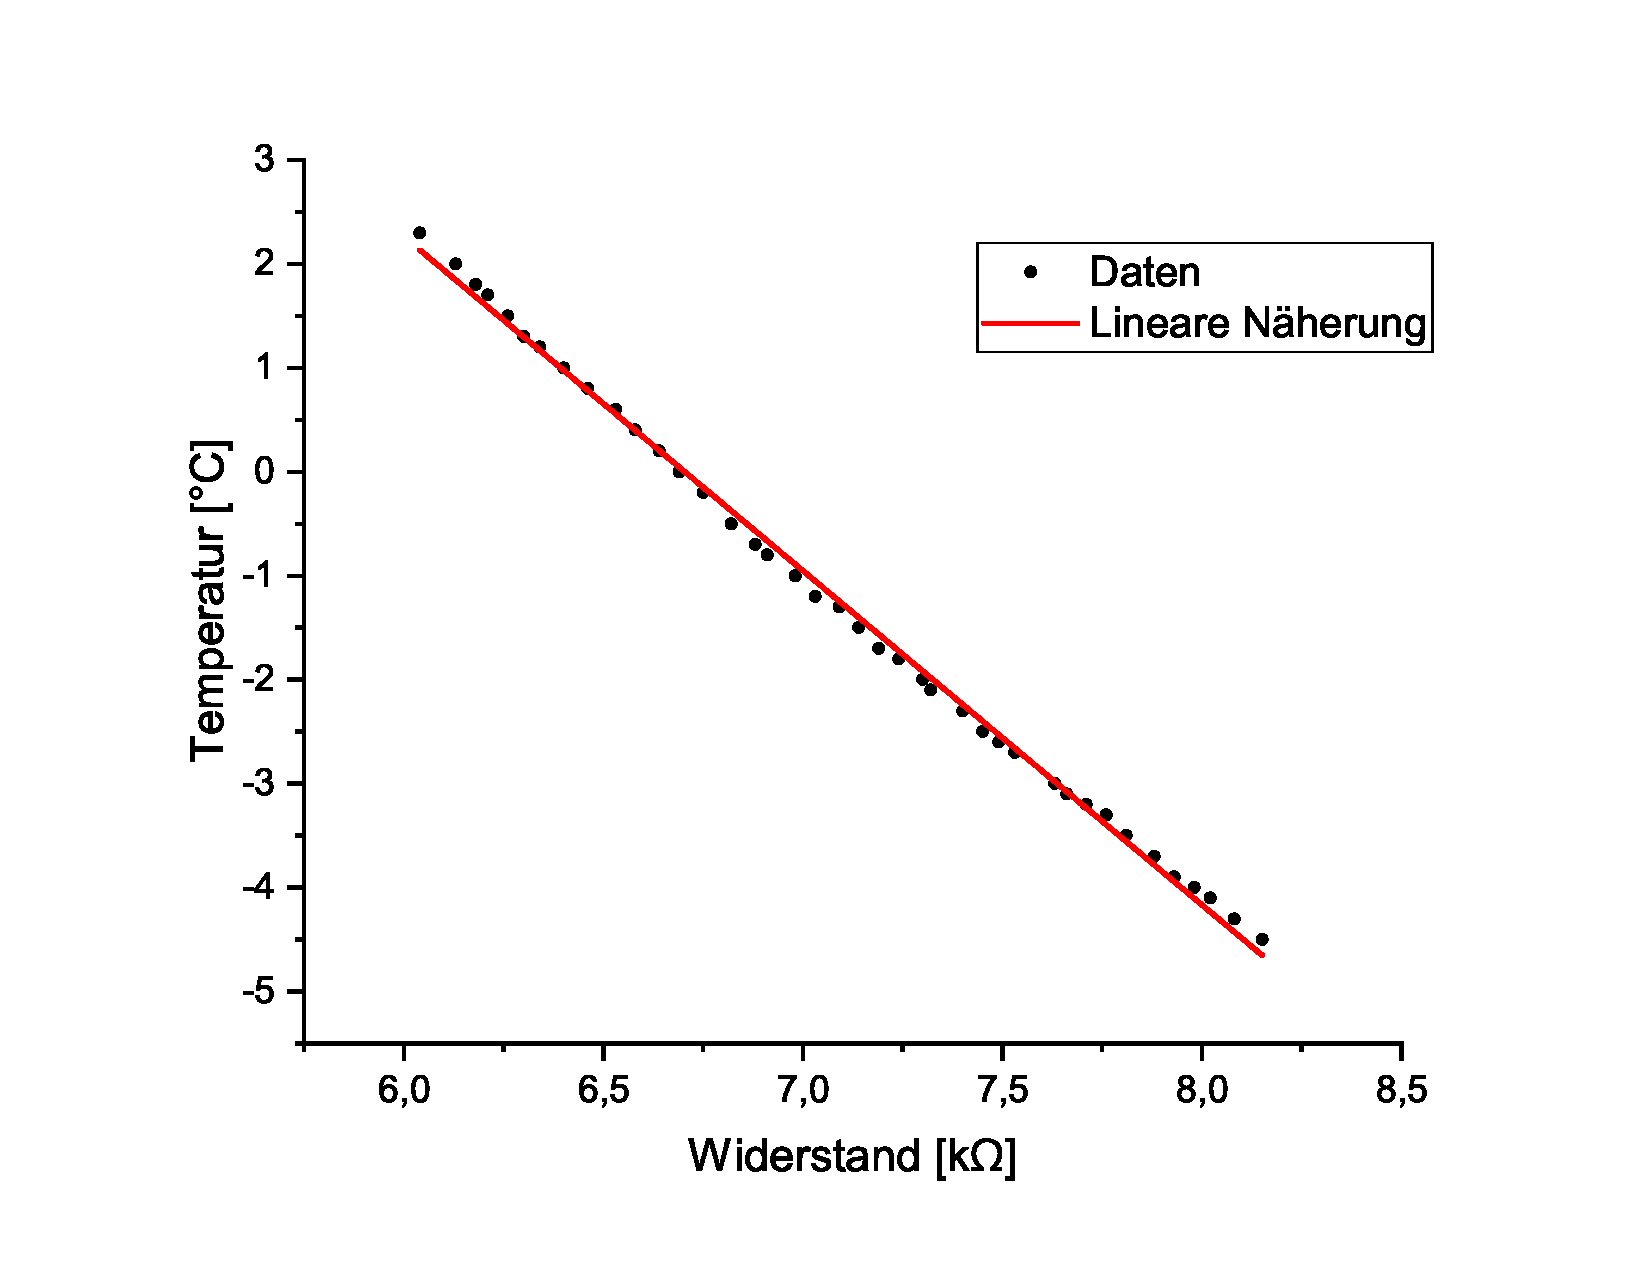
\includegraphics[scale=0.5]{Bilder/Kalibrierung_Termistor.eps}
        \caption{Widerstand-Temperatur-Diagramm}
    \end{center}
\end{figure}


\subsection{Widerstandskurven des Termistors}

\begin{figure}
    \begin{tikzpicture}
    \begin{axis}[
    height=\plotheight, width=\plotwidth,
    xlabel={$t$ in $\unit{s}$}, ylabel={$R$ in $\unit{k\Omega}$},
    xmin=-10, xmax=270, only marks,
    legend entries={1. Messreihe, 2. Messreihe, 3. Messreihe}, legend pos=south east,
    ]
    \addplot table [x=t, y=R, col sep=comma] {./Daten/wasser1.csv};
    \addplot table [x=t, y=R, col sep=comma] {./Daten/wasser2.csv};
    \addplot+[mark=triangle*, mark options={fill=green}, color=green, mark size=3] table [x=t, y=R, col sep=comma] {./Daten/wasser3.csv};
    \addplot+[domain=-10:320, smooth, mark=, dashed, very thick] {6.6633};
    \end{axis}
    \end{tikzpicture}
    
    \caption{Gefrierpunktmessung destilliertes Wasser}
    \label{diag:wasser}
\end{figure}

\begin{figure}    
    \begin{tikzpicture}
    \begin{axis}[
    height=\plotheight, width=\plotwidth,
    xlabel={$t$ in $\unit{s}$}, ylabel={$R$ in $\unit{k\Omega}$},
    xmin=-10, xmax=800, only marks,
    legend entries={1. Messreihe, 2. Messreihe, 3. Messreihe}, legend pos=south east,
    ]
    \addplot+[mark size=1] table [x=t, y=R, col sep=comma] {./Daten/salz1.csv};
    \addplot+[mark size=1] table [x=t, y=R, col sep=comma] {./Daten/salz2.csv};
    \addplot+[mark=triangle*, mark options={fill=green}, color=green, mark size=2] table [x=t, y=R, col sep=comma] {./Daten/salz3.csv};
    \addplot+[domain=-10:800, smooth, mark=, dashed, very thick] {7.0233};
    \end{axis}
    \end{tikzpicture}
    
    \caption{Gefrierpunktmessung Salzlösung}
    \label{diag:salz}
\end{figure}

Abbildungen ~\ref{diag:wasser} und \ref{diag:salz} zeige die zeitliche Entwicklung des Widerstands des Termistor während der Abkühlung der Probe. Sie stimmen deutlich mit der in der Aufgabenstellung skizzierten Modellkurve überein (der Abfall nach dem Peak ist bei unseren Messungen jedoch steiler und tritt sehr plötzlich ein). 
Da die Parameter der Abkühlung für das Experiment irrelevant sind wurden sie nicht kontrolliert, deshalb unterscheidet sich die genau zeitliche Entwicklung des Widerstandes stark. Insbesondere war bei der 2. Messreihe mit der Salzlösung das Kältebad relativ warm, weshalb es lange gedauert hat bis die Lösung gefroren ist.

Wir erhalten für die Widerstände des Termistors bei Schmelztemperatur jeweils $R_\mathrm{G} = \unit[(6.663 \pm 0.004)]{k\Omega}$ und $R_\mathrm{G1} = \unit[(7.023 \pm 0.004)]{k\Omega}$ (vgl. Abb.~\ref{diag:wasser} und \ref{diag:salz})

\subsection{Bestimmung des Dissoziationsgrades}

Wir erhalten für die entsprechenden Gefrierpunkte $T_\mathrm{G} \approx \unit[0.1]{ ^\circ C}$ und $T_\mathrm{G1} \approx \unit[-1.0]{ ^\circ C}$. Die Für die Auswertung wichtige Temperaturdifferenz berechnet sich aus
\begin{align}
    \Delta T_\mathrm{G} &= a (R_\mathrm{G} - R_\mathrm{G1}) \label{eq:DT} \\
                        &= \unit[1.157 \pm 0.020]{K} \notag
\end{align} 
insbesondere unabhängig vom Regressionsparameter $b$, weshalb der Fehler hier relativ klein ist.
%
Aus Gleichung~\ref{eq:N'} folgt mit der abgewogenen Wassermenge $n M_1 = \unit[(20.1709 \pm 0.0011)]{g}$
\[
    N' = \unit[(0.01256 \pm 0.00022)]{mol}
\]
%
Gleichung~\ref{eq:alpha} liefert mit $N = \unit[(0.5700 \pm 0.0007)]{g} / \unit[84.99]{g\,mol^{-1}} = \unit[(6.707 \pm 0.008)]{mol}$ an gelöstem Salz und $z = 2$ den Wert 
\[
    \alpha = 0.873 \pm 0.016
\]










